\documentclass[]{elsarticle} %review=doublespace preprint=single 5p=2 column
%%% Begin My package additions %%%%%%%%%%%%%%%%%%%
\usepackage[hyphens]{url}

  \journal{SportR\(\chi\)iv} % Sets Journal name


\usepackage{lineno} % add
\providecommand{\tightlist}{%
  \setlength{\itemsep}{0pt}\setlength{\parskip}{0pt}}

\usepackage{graphicx}
\usepackage{booktabs} % book-quality tables
%%%%%%%%%%%%%%%% end my additions to header

\usepackage[T1]{fontenc}
\usepackage{lmodern}
\usepackage{amssymb,amsmath}
\usepackage{ifxetex,ifluatex}
\usepackage{fixltx2e} % provides \textsubscript
% use upquote if available, for straight quotes in verbatim environments
\IfFileExists{upquote.sty}{\usepackage{upquote}}{}
\ifnum 0\ifxetex 1\fi\ifluatex 1\fi=0 % if pdftex
  \usepackage[utf8]{inputenc}
\else % if luatex or xelatex
  \usepackage{fontspec}
  \ifxetex
    \usepackage{xltxtra,xunicode}
  \fi
  \defaultfontfeatures{Mapping=tex-text,Scale=MatchLowercase}
  \newcommand{\euro}{€}
\fi
% use microtype if available
\IfFileExists{microtype.sty}{\usepackage{microtype}}{}
\bibliographystyle{elsarticle-harv}
\ifxetex
  \usepackage[setpagesize=false, % page size defined by xetex
              unicode=false, % unicode breaks when used with xetex
              xetex]{hyperref}
\else
  \usepackage[unicode=true]{hyperref}
\fi
\hypersetup{breaklinks=true,
            bookmarks=true,
            pdfauthor={},
            pdftitle={Short Paper},
            colorlinks=false,
            urlcolor=blue,
            linkcolor=magenta,
            pdfborder={0 0 0}}
\urlstyle{same}  % don't use monospace font for urls

\setcounter{secnumdepth}{0}
% Pandoc toggle for numbering sections (defaults to be off)
\setcounter{secnumdepth}{0}

\newlength{\cslhangindent}
\setlength{\cslhangindent}{1.5em}
\newenvironment{cslreferences}%
  {\setlength{\parindent}{0pt}%
  \everypar{\setlength{\hangindent}{\cslhangindent}}\ignorespaces}%
  {\par}

% Pandoc header
\usepackage{booktabs}
\usepackage{longtable}
\usepackage{array}
\usepackage{multirow}
\usepackage{wrapfig}
\usepackage{float}
\usepackage{colortbl}
\usepackage{pdflscape}
\usepackage{tabu}
\usepackage{threeparttable}
\usepackage{threeparttablex}
\usepackage[normalem]{ulem}
\usepackage{makecell}
\usepackage{xcolor}



\begin{document}
\begin{frontmatter}

  \title{Short Paper}
    \author[Centre for Sport Research]{Aaron S. Fox\corref{1}}
  
    \author[Centre for Sport Research]{Tanisha Bardzinski}
  
    \author[Centre for Sport Research]{Lyndell Bruce}
  
      \address[Centre for Sport Research]{Centre for Sport Research,
School of Exercise and Nutrition Sciences, Deakin University, Geelong,
Australia}
      \cortext[1]{Corresponding Author: aaron.f@deakin.edu.au}
  
  \begin{abstract}
  Insert abstract\ldots{}
  \end{abstract}
  
 \end{frontmatter}

\hypertarget{introduction}{%
\section{Introduction}\label{introduction}}

Netball is a court-based team sport played predominantly among
Commonwealth nations, and has one of the highest participation rates for
team sports in Australia ({\textbf{???}}). As in many court-based team
sports, the goal of netball is to score more than the opposition.
Netball is, however, unique in that goals may only be scored by two
players on each team from within the `shooting circle' (i.e.~a half
circle around the goal with a 4.9m radius) at their end of the court
({\textbf{???}}). Traditionally, goals scored from within this circle
result in one `goal' or `point' for the team ({\textbf{???}}). In the
2020 season, Australia's national elite-level league (i.e.~Suncorp Super
Netball) made the decision to introduce the `Super Shot'
({\textbf{???}}). The Super Shot period provided teams an opportunity to
gain one- versus two-points for successful shots made from the `inner'
(i.e.~0m-3.0m) versus `outer' (i.e.~3.0m-4.9m), respectively, within the
final five minutes of each quarter ({\textbf{???}}). The league has
confirmed that the Super Shot rule will continue through the 2021 season
({\textbf{???}}).

Our analysis prior to the 2020 season ({\textbf{???}}) suggested that
the added value of the Super Shot (i.e.~two-points) aligned well with
the elevated risk of shooting from long range, and that teams may have
been able to maximise their scoring by taking a high proportion of Super
Shots. These findings were, however, based on shooting statistics from
past seasons where the Super Shot rule was not in effect -- and further
investigation of leagues where a `two-point rule' was in place
(i.e.~international Fast5) resulted in a much higher risk of missing
long-range shots ({\textbf{???}}). We hypothesised that the elevated
risk of missing long-range shots with a `two-point rule' in place stems
from situational factors, whereby defensive strategies were likely
altered to place a heavier emphasis on defending long-range shots
({\textbf{???}}). Data from the first full season with the Super Shot in
place provides an opportunity to re-evaluate the risk-reward value of
taking Super Shots with more valid shooting statistics. Further, these
data can provide a better foundation for simulating Super Shot periods
as a means to identify optimal shooting strategies. In the present study
we re-visited the question of whether the weighting of a 2:1 value is
appropriate based on the relative risk of missing a shot from the outer
versus inner circle during the Super Shot period using data from the
2020 season. Further -- we ran a series of simulations of the
five-minute Super Shot period, driven by shooting statistics from the
2020 season, in an attempt to identify optimal team-specific shooting
strategies for the proportion of Super Shots to take.

\hypertarget{methods}{%
\section{Methods}\label{methods}}

\hypertarget{participants}{%
\subsection{Participants}\label{participants}}

Participants for this study included all players across the eight teams
from the 2020 season of the Australian national netball league
(i.e.~Suncorp Super Netball). Our study included publicly available,
pre-existing data held on the Suncorp Super Netball match centre
(\textbf{\emph{TODO: add link}}). An exemption from ethics review (and
subsequent waiver of individual consent) was granted by the Deakin
University Human Research Ethics Committee (\textbf{\emph{TODO: add
details}}).

\hypertarget{data-collection}{%
\subsection{Data Collection}\label{data-collection}}

We used the \{SuperNetballR\}\textbf{\emph{TODO: citation}} package to
extract match data from all regular season games during the 2020 Super
Netball Season via the Champion Data (official provider of competition
statistics) match centre. Within the match centre data -- all shots are
labelled with identifiers that place them in the inner or outer circle,
along with whether they were made or missed. Combined with the timestamp
of these events within quarters, we extracted team-specific shooting
statistics for: (i) the total number of shots taken; (ii) the number of
shots taken from the inner and outer circle; and (iii) the number of
made and missed shots from the inner and outer circle from each Super
Shot period across the season.

\hypertarget{data-analysis}{%
\subsection{Data Analysis}\label{data-analysis}}

Our study required estimating the probability of making versus missing
shots from the inner versus outer circle across the different teams. We
achieved this by defining a beta distribution in a probability density
function for the different circle zones, specified by:

\textbf{\emph{TODO: add math function}}

where \emph{a} and \emph{b} represent the number of missed and made
shots within a circle zone, respectively; \textbf{\emph{TODO: add x math
symbol}} is the probability of \emph{a} relative to \emph{b}; and
\textbf{\emph{TODO: add gamma}} is the gamma function ({\textbf{???}}).
Probability density functions were created for made versus missed shots
in the inner and outer circles for each team, as well as all teams
combined, to be used in subsequent analyses.

To examine the relative value of the 2:1 point ratio, we replicated the
approach from our previous work ({\textbf{???}}) but this time with data
from the 2020 season. Specifically, we compared the average relative
odds (± 95\% confidence intervals {[}CI{]}) of missing from the outer
versus inner circle during the Super Shot period. This was achieved by
dividing randomly sampled values (\emph{n} = 1,000) from the probability
density functions of the outer by those from the inner circle at each
sample iteration. This analysis was run using shooting statistics from
the entire league, as well as individual teams, to give overall and
team-specific risk-reward values for attempting Super Shots.
Theoretically, the relative odds of missing from the outer to inner
circle should match the ratio of points awarded (i.e.~2:1) for the Super
Shot to represent `good value.'

\textbf{\emph{TODO: add defensive calculations too\ldots{}}}

\ldots{}

\ldots combination of coded and publicly available data\ldots{}

Our approach in the present paper to simulate Super Shot scoring periods
differs to our original work ({\textbf{???}}). Previously, we allocated
an overall success rate to shots from the inner versus outer circle
(i.e.~if the sampled probability was 50\%, a total of 50\% of shots were
counted as successful). This contrasts to our present work, where we
sample and apply the probability of shot success to simulated individual
shots (i.e.~if the sampled probability is 50\%, the individual shot
being simulated has a 50\% probability of success). This approach likely
reflects an improvement on our analysis, better representing the
independent nature of shots in a netball match.

\begin{itemize}
\tightlist
\item
  Include some probability calculations of winning vs.~losing the 5
  minute period (i.e.~X team's relative probability of winning
  vs.~losing the super shot period under different proportions; or maybe
  even between proportions?)
\end{itemize}

\hypertarget{results}{%
\section{Results}\label{results}}

The relative combined odds (± 95\% CIs) from all teams of missing from
the outer versus the inner circle across the entire match were 4.19
{[}3.88, 4.52{]}, and 4.04 {[}3.5, 4.6{]} versus 4.68 {[}4.07, 5.35{]}
in the standard and Super Shot periods, respectively. The relative odds
of missing from the outer versus inner circle across the individual
teams were relatively similar, with the exception of the Fever having
higher odds than the majority of teams across all match periods (see
Figure \ref{fig:relativeOddsFig}). The relative odds (± 95\% CIs) of
missing from the outer versus inner circle during the Super Shot Period
were greater than 2:1 across all teams (see Figure
\ref{fig:relativeOddsFig}). No team was more effective in elevating the
risk of missing from the outer versus inner circle, with mostly similar
odds observed across all teams opponents in the various periods of the
quarter (see Figure \ref{fig:relativeOddsDefFig}).

\begin{figure}
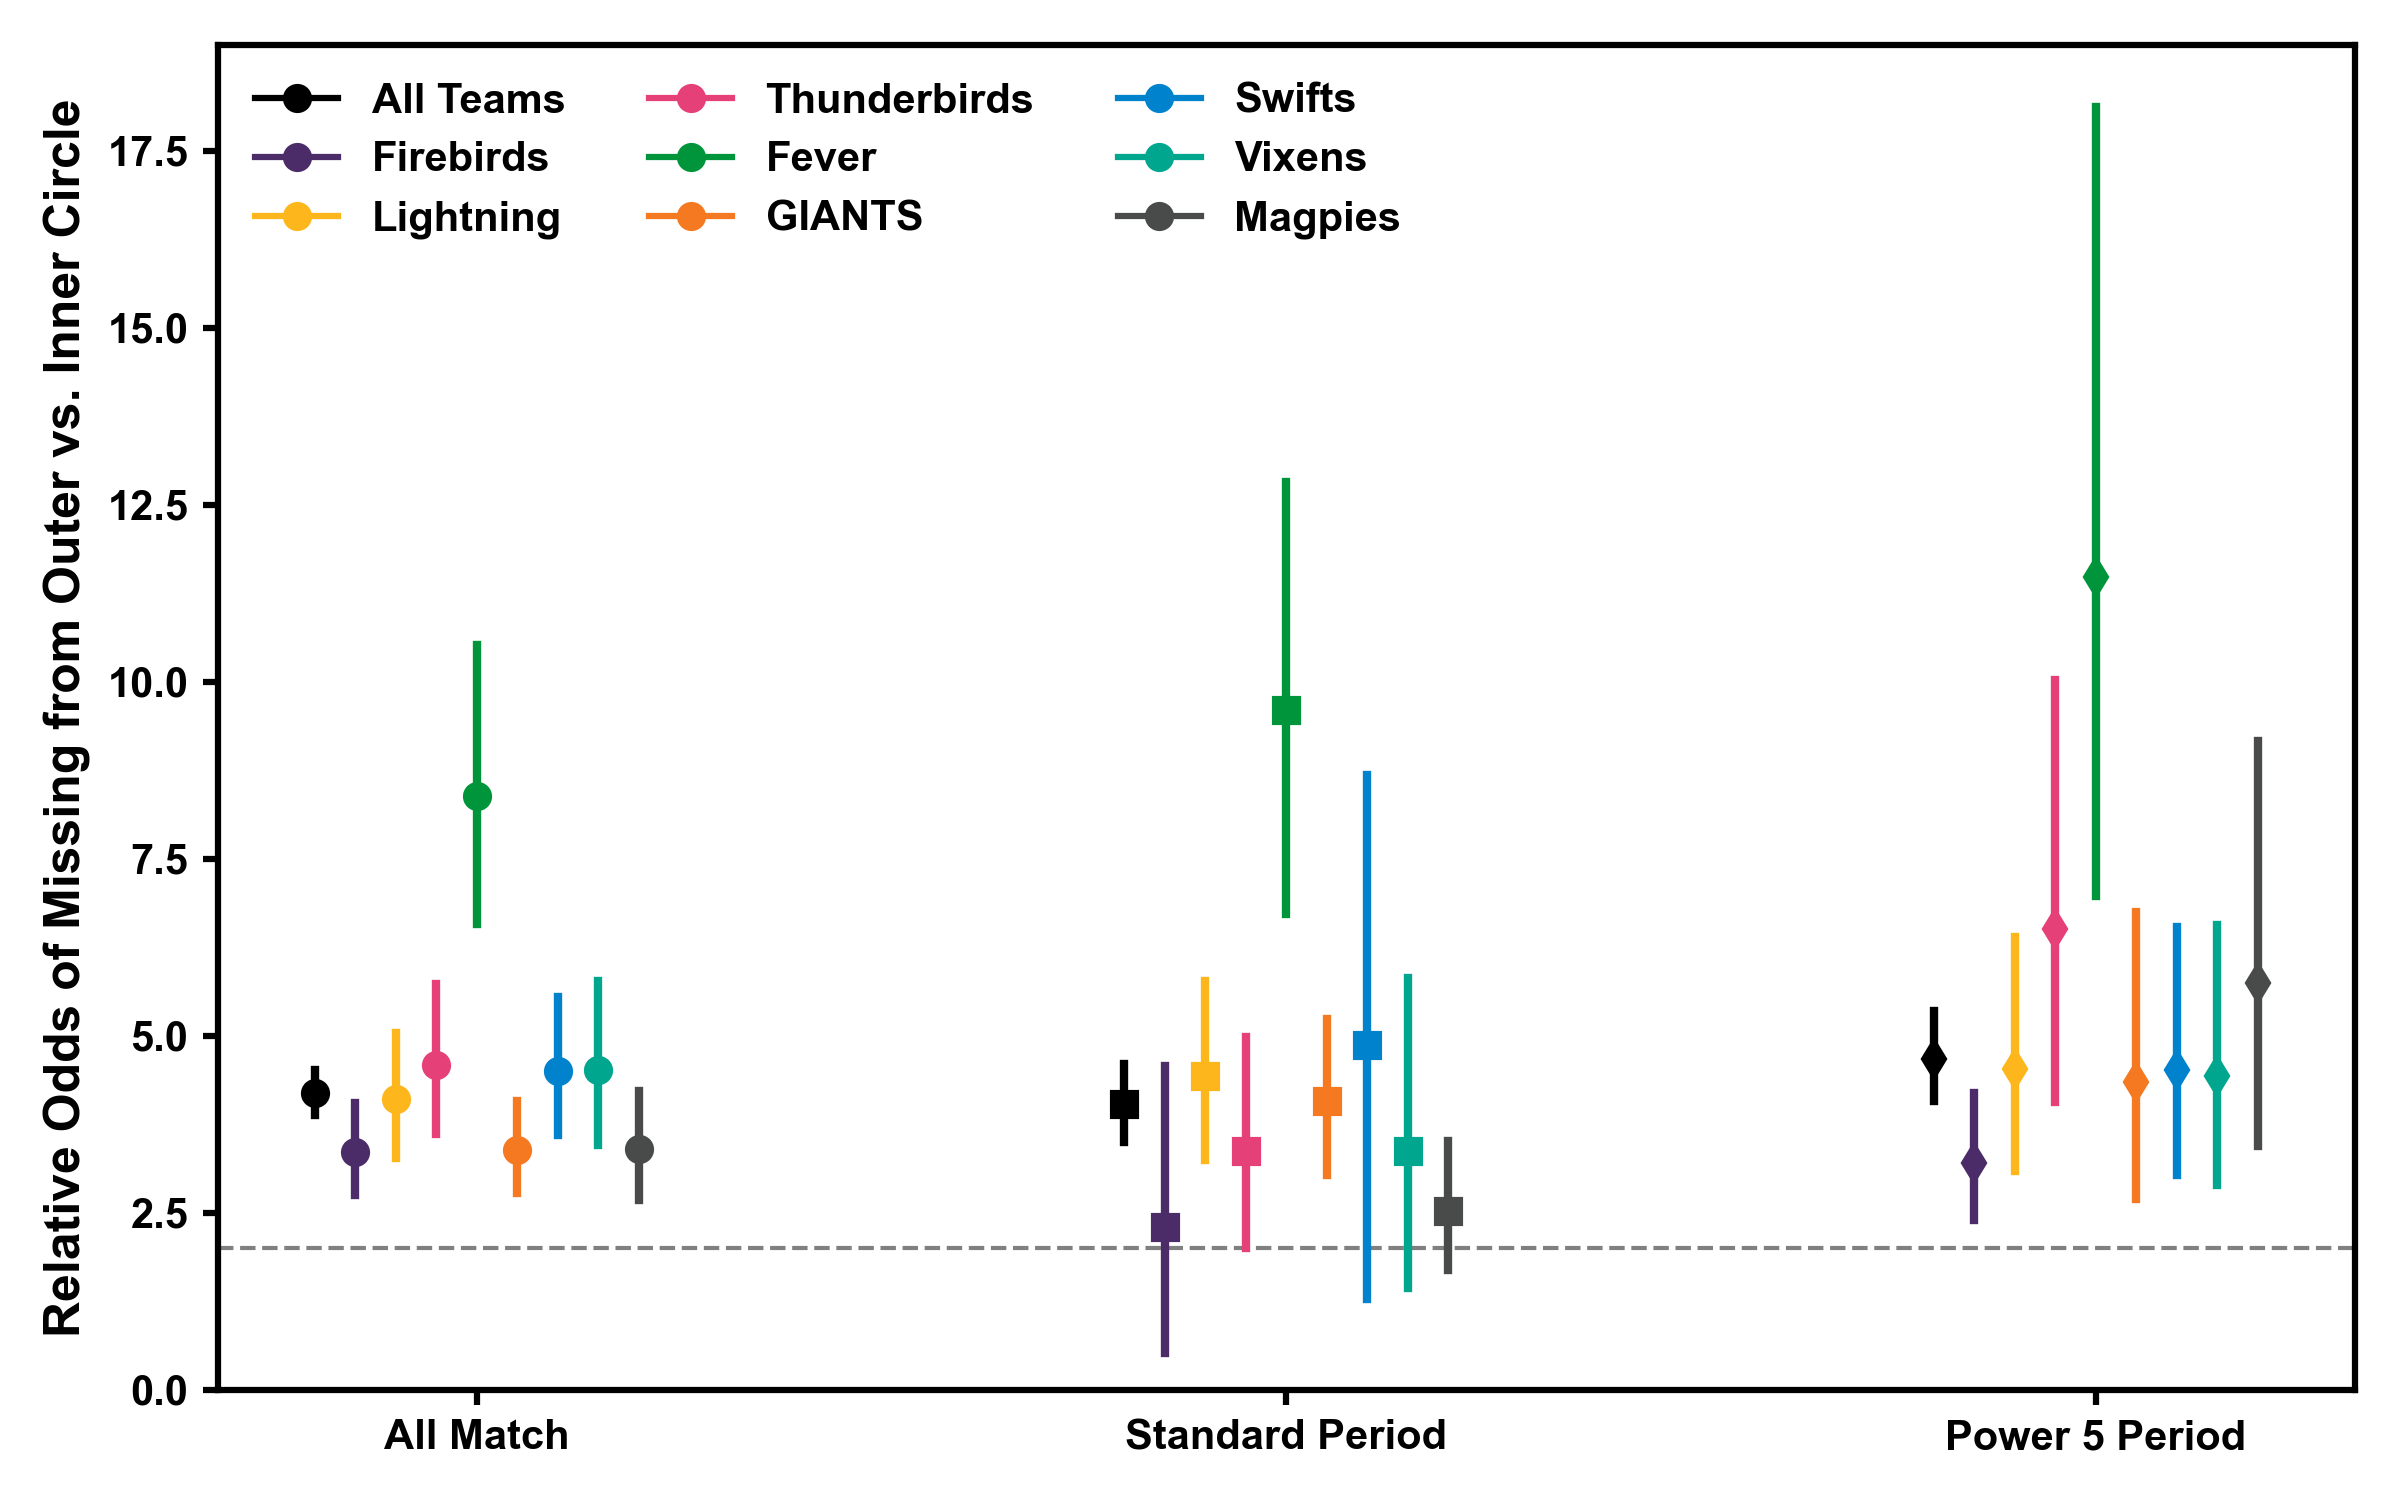
\includegraphics[width=0.5\linewidth]{D:/+GitRepos+/super-shot-sims/Results/relativeOdds/figures/RelativeOdds_OuterInner_AllTeams} \caption{A caption}\label{fig:relativeOddsFig}
\end{figure}

\begin{figure}
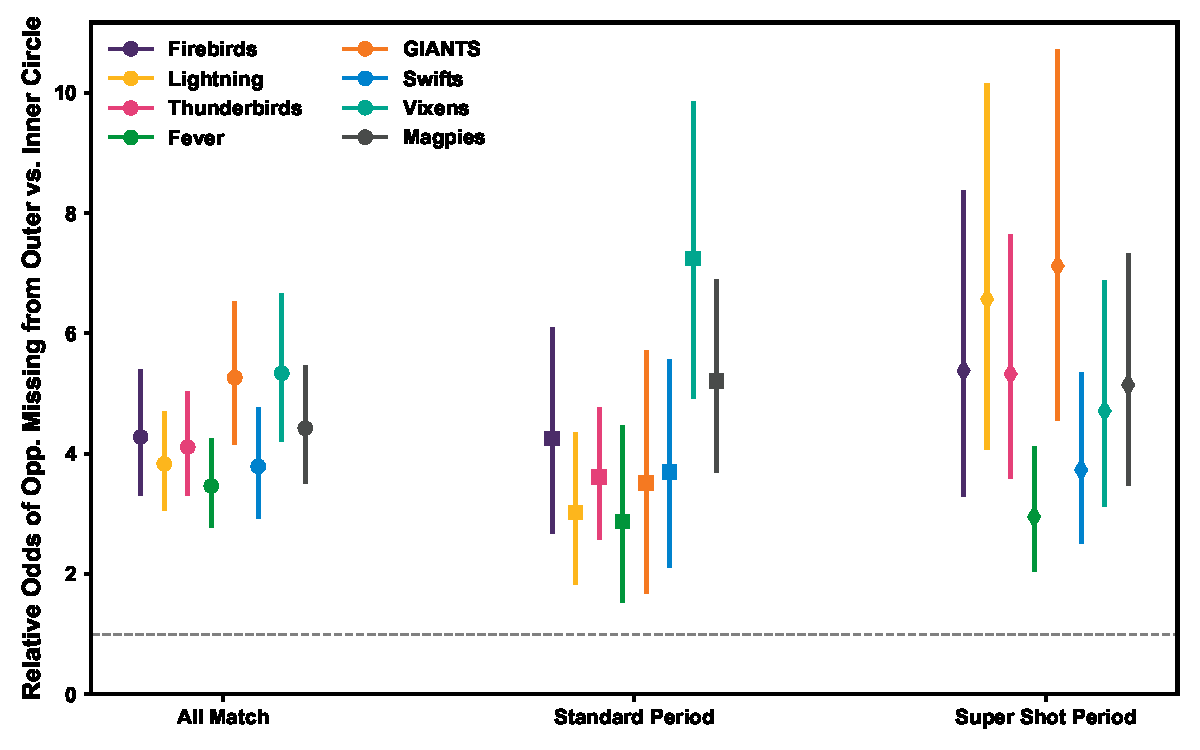
\includegraphics[width=0.5\linewidth]{D:/+GitRepos+/super-shot-sims/Results/relativeOdds/figures/RelativeOddsDef_OuterInner_AllTeams} \caption{A caption}\label{fig:relativeOddsDefFig}
\end{figure}

\ldots{}

\begin{landscape}\begin{table}

\caption{\label{tab:marginTable}Table X: TODO Add caption}
\centering
\resizebox{\linewidth}{!}{
\begin{tabular}[t]{lllllllll}
\toprule
X & Fever & Firebirds & GIANTS & Lightning & Magpies & Swifts & Thunderbirds & Vixens\\
\midrule
\cellcolor{gray!6}{Team 0\% / Opp. 0\%} & \cellcolor{gray!6}{0.25 [0.06, 0.45]} & \cellcolor{gray!6}{-0.51 [-0.70, -0.32]} & \cellcolor{gray!6}{-0.10 [-0.29, 0.09]} & \cellcolor{gray!6}{-0.01 [-0.20, 0.19]} & \cellcolor{gray!6}{0.13 [-0.07, 0.32]} & \cellcolor{gray!6}{-0.01 [-0.21, 0.18]} & \cellcolor{gray!6}{0.13 [-0.06, 0.33]} & \cellcolor{gray!6}{0.12 [-0.07, 0.31]}\\
Team 0\% / Opp. 25\% & 0.21 [0.00, 0.41] & -0.29 [-0.50, -0.09] & 0.33 [0.12, 0.54] & 0.27 [0.06, 0.49] & 0.46 [0.24, 0.67] & 0.25 [0.04, 0.47] & 0.31 [0.10, 0.53] & 0.54 [0.32, 0.76]\\
\cellcolor{gray!6}{Team 0\% / Opp. 50\%} & \cellcolor{gray!6}{0.19 [-0.03, 0.40]} & \cellcolor{gray!6}{-0.02 [-0.25, 0.20]} & \cellcolor{gray!6}{0.71 [0.47, 0.94]} & \cellcolor{gray!6}{0.56 [0.33, 0.79]} & \cellcolor{gray!6}{0.78 [0.54, 1.01]} & \cellcolor{gray!6}{0.49 [0.26, 0.73]} & \cellcolor{gray!6}{0.51 [0.27, 0.74]} & \cellcolor{gray!6}{0.97 [0.73, 1.21]}\\
Team 0\% / Opp. 75\% & 0.07 [-0.16, 0.30] & 0.13 [-0.11, 0.36] & 1.10 [0.86, 1.35] & 0.77 [0.53, 1.01] & 1.04 [0.80, 1.28] & 0.75 [0.51, 0.99] & 0.70 [0.46, 0.94] & 1.37 [1.12, 1.62]\\
\cellcolor{gray!6}{Team 0\% / Opp. 100\%} & \cellcolor{gray!6}{-0.06 [-0.30, 0.19]} & \cellcolor{gray!6}{0.28 [0.03, 0.52]} & \cellcolor{gray!6}{1.49 [1.22, 1.75]} & \cellcolor{gray!6}{1.02 [0.76, 1.27]} & \cellcolor{gray!6}{1.31 [1.05, 1.57]} & \cellcolor{gray!6}{0.95 [0.69, 1.20]} & \cellcolor{gray!6}{0.75 [0.50, 1.01]} & \cellcolor{gray!6}{1.64 [1.38, 1.90]}\\
\addlinespace
Team 25\% / Opp. 0\% & -0.04 [-0.26, 0.18] & -0.77 [-0.98, -0.56] & -0.33 [-0.54, -0.12] & -0.27 [-0.48, -0.05] & -0.13 [-0.34, 0.09] & -0.28 [-0.49, -0.07] & -0.14 [-0.35, 0.07] & -0.12 [-0.33, 0.09]\\
\cellcolor{gray!6}{Team 25\% / Opp. 25\%} & \cellcolor{gray!6}{-0.09 [-0.31, 0.14]} & \cellcolor{gray!6}{-0.55 [-0.77, -0.32]} & \cellcolor{gray!6}{0.10 [-0.13, 0.33]} & \cellcolor{gray!6}{0.02 [-0.21, 0.25]} & \cellcolor{gray!6}{0.20 [-0.03, 0.43]} & \cellcolor{gray!6}{-0.01 [-0.24, 0.22]} & \cellcolor{gray!6}{0.03 [-0.19, 0.26]} & \cellcolor{gray!6}{0.30 [0.07, 0.53]}\\
Team 25\% / Opp. 50\% & -0.11 [-0.35, 0.13] & -0.28 [-0.52, -0.04] & 0.48 [0.22, 0.73] & 0.30 [0.05, 0.55] & 0.52 [0.27, 0.77] & 0.23 [-0.02, 0.48] & 0.23 [-0.02, 0.48] & 0.73 [0.47, 0.98]\\
\cellcolor{gray!6}{Team 25\% / Opp. 75\%} & \cellcolor{gray!6}{-0.22 [-0.47, 0.03]} & \cellcolor{gray!6}{-0.13 [-0.38, 0.12]} & \cellcolor{gray!6}{0.87 [0.61, 1.13]} & \cellcolor{gray!6}{0.51 [0.26, 0.77]} & \cellcolor{gray!6}{0.79 [0.53, 1.05]} & \cellcolor{gray!6}{0.49 [0.23, 0.74]} & \cellcolor{gray!6}{0.42 [0.17, 0.67]} & \cellcolor{gray!6}{1.13 [0.87, 1.39]}\\
Team 25\% / Opp. 100\% & -0.35 [-0.62, -0.09] & 0.02 [-0.24, 0.28] & 1.25 [0.98, 1.53] & 0.76 [0.49, 1.03] & 1.05 [0.78, 1.33] & 0.68 [0.41, 0.95] & 0.48 [0.21, 0.74] & 1.40 [1.12, 1.67]\\
\addlinespace
\cellcolor{gray!6}{Team 50\% / Opp. 0\%} & \cellcolor{gray!6}{-0.34 [-0.58, -0.10]} & \cellcolor{gray!6}{-1.04 [-1.27, -0.80]} & \cellcolor{gray!6}{-0.57 [-0.81, -0.34]} & \cellcolor{gray!6}{-0.52 [-0.75, -0.29]} & \cellcolor{gray!6}{-0.37 [-0.60, -0.14]} & \cellcolor{gray!6}{-0.54 [-0.77, -0.31]} & \cellcolor{gray!6}{-0.42 [-0.65, -0.19]} & \cellcolor{gray!6}{-0.37 [-0.60, -0.15]}\\
Team 50\% / Opp. 25\% & -0.38 [-0.63, -0.13] & -0.81 [-1.06, -0.57] & -0.15 [-0.40, 0.10] & -0.24 [-0.49, 0.01] & -0.05 [-0.30, 0.20] & -0.28 [-0.52, -0.03] & -0.24 [-0.49, 0.01] & 0.05 [-0.20, 0.29]\\
\cellcolor{gray!6}{Team 50\% / Opp. 50\%} & \cellcolor{gray!6}{-0.40 [-0.67, -0.14]} & \cellcolor{gray!6}{-0.54 [-0.81, -0.28]} & \cellcolor{gray!6}{0.23 [-0.04, 0.50]} & \cellcolor{gray!6}{0.05 [-0.22, 0.31]} & \cellcolor{gray!6}{0.27 [0.00, 0.54]} & \cellcolor{gray!6}{-0.03 [-0.30, 0.23]} & \cellcolor{gray!6}{-0.05 [-0.31, 0.22]} & \cellcolor{gray!6}{0.48 [0.21, 0.75]}\\
Team 50\% / Opp. 75\% & -0.52 [-0.78, -0.26] & -0.40 [-0.66, -0.13] & 0.63 [0.35, 0.91] & 0.26 [-0.01, 0.53] & 0.54 [0.27, 0.81] & 0.22 [-0.05, 0.49] & 0.15 [-0.12, 0.41] & 0.88 [0.60, 1.15]\\
\cellcolor{gray!6}{Team 50\% / Opp. 100\%} & \cellcolor{gray!6}{-0.65 [-0.93, -0.37]} & \cellcolor{gray!6}{-0.24 [-0.52, 0.03]} & \cellcolor{gray!6}{1.01 [0.72, 1.30]} & \cellcolor{gray!6}{0.51 [0.22, 0.79]} & \cellcolor{gray!6}{0.81 [0.52, 1.10]} & \cellcolor{gray!6}{0.42 [0.13, 0.71]} & \cellcolor{gray!6}{0.20 [-0.08, 0.48]} & \cellcolor{gray!6}{1.15 [0.86, 1.44]}\\
\addlinespace
Team 75\% / Opp. 0\% & -0.62 [-0.86, -0.38] & -1.26 [-1.50, -1.03] & -0.77 [-1.01, -0.53] & -0.75 [-0.99, -0.50] & -0.59 [-0.83, -0.35] & -0.75 [-0.99, -0.51] & -0.63 [-0.87, -0.39] & -0.55 [-0.79, -0.31]\\
\cellcolor{gray!6}{Team 75\% / Opp. 25\%} & \cellcolor{gray!6}{-0.66 [-0.92, -0.41]} & \cellcolor{gray!6}{-1.04 [-1.29, -0.79]} & \cellcolor{gray!6}{-0.34 [-0.60, -0.09]} & \cellcolor{gray!6}{-0.46 [-0.72, -0.21]} & \cellcolor{gray!6}{-0.27 [-0.52, -0.01]} & \cellcolor{gray!6}{-0.49 [-0.75, -0.23]} & \cellcolor{gray!6}{-0.46 [-0.71, -0.20]} & \cellcolor{gray!6}{-0.13 [-0.39, 0.13]}\\
Team 75\% / Opp. 50\% & -0.69 [-0.95, -0.42] & -0.77 [-1.04, -0.51] & 0.04 [-0.24, 0.31] & -0.18 [-0.45, 0.09] & 0.05 [-0.22, 0.33] & -0.25 [-0.52, 0.03] & -0.26 [-0.54, 0.01] & 0.30 [0.02, 0.58]\\
\cellcolor{gray!6}{Team 75\% / Opp. 75\%} & \cellcolor{gray!6}{-0.80 [-1.07, -0.53]} & \cellcolor{gray!6}{-0.63 [-0.90, -0.35]} & \cellcolor{gray!6}{0.43 [0.15, 0.72]} & \cellcolor{gray!6}{0.03 [-0.25, 0.31]} & \cellcolor{gray!6}{0.32 [0.04, 0.60]} & \cellcolor{gray!6}{0.01 [-0.27, 0.29]} & \cellcolor{gray!6}{-0.07 [-0.35, 0.21]} & \cellcolor{gray!6}{0.70 [0.41, 0.99]}\\
Team 75\% / Opp. 100\% & -0.93 [-1.21, -0.65] & -0.47 [-0.75, -0.19] & 0.81 [0.52, 1.11] & 0.28 [-0.01, 0.57] & 0.59 [0.29, 0.88] & 0.21 [-0.09, 0.50] & -0.01 [-0.30, 0.28] & 0.97 [0.67, 1.27]\\
\addlinespace
\cellcolor{gray!6}{Team 100\% / Opp. 0\%} & \cellcolor{gray!6}{-0.80 [-1.06, -0.53]} & \cellcolor{gray!6}{-1.41 [-1.67, -1.16]} & \cellcolor{gray!6}{-0.90 [-1.15, -0.64]} & \cellcolor{gray!6}{-0.91 [-1.16, -0.65]} & \cellcolor{gray!6}{-0.77 [-1.03, -0.51]} & \cellcolor{gray!6}{-0.96 [-1.21, -0.70]} & \cellcolor{gray!6}{-0.87 [-1.12, -0.61]} & \cellcolor{gray!6}{-0.77 [-1.02, -0.51]}\\
Team 100\% / Opp. 25\% & -0.84 [-1.11, -0.57] & -1.19 [-1.46, -0.92] & -0.47 [-0.74, -0.20] & -0.62 [-0.90, -0.35] & -0.44 [-0.71, -0.17] & -0.69 [-0.97, -0.42] & -0.69 [-0.96, -0.42] & -0.35 [-0.62, -0.07]\\
\cellcolor{gray!6}{Team 100\% / Opp. 50\%} & \cellcolor{gray!6}{-0.86 [-1.14, -0.58]} & \cellcolor{gray!6}{-0.92 [-1.20, -0.64]} & \cellcolor{gray!6}{-0.09 [-0.38, 0.20]} & \cellcolor{gray!6}{-0.34 [-0.63, -0.05]} & \cellcolor{gray!6}{-0.12 [-0.41, 0.17]} & \cellcolor{gray!6}{-0.45 [-0.74, -0.16]} & \cellcolor{gray!6}{-0.50 [-0.78, -0.21]} & \cellcolor{gray!6}{0.08 [-0.21, 0.38]}\\
Team 100\% / Opp. 75\% & -0.98 [-1.27, -0.69] & -0.77 [-1.06, -0.48] & 0.30 [0.01, 0.60] & -0.13 [-0.42, 0.17] & 0.14 [-0.15, 0.44] & -0.19 [-0.48, 0.10] & -0.30 [-0.59, -0.01] & 0.48 [0.19, 0.78]\\
\cellcolor{gray!6}{Team 100\% / Opp. 100\%} & \cellcolor{gray!6}{-1.11 [-1.41, -0.81]} & \cellcolor{gray!6}{-0.62 [-0.92, -0.32]} & \cellcolor{gray!6}{0.69 [0.38, 1.00]} & \cellcolor{gray!6}{0.12 [-0.19, 0.43]} & \cellcolor{gray!6}{0.41 [0.10, 0.72]} & \cellcolor{gray!6}{0.00 [-0.30, 0.31]} & \cellcolor{gray!6}{-0.25 [-0.55, 0.06]} & \cellcolor{gray!6}{0.75 [0.44, 1.07]}\\
\bottomrule
\end{tabular}}
\end{table}
\end{landscape}

\hypertarget{discussion}{%
\section{Discussion}\label{discussion}}

\ldots{}

Discussion points\ldots{} - Consideration around our newly calculated
relative risk of missing with respect to point value. Higher than
previous, so now is the Super Shot worth taking? We could also do this
specifically against a team as well as overall (i.e.~what is the
relative risk of make vs.~miss for specific teams or against specific
teams) - General/overall value with respect to different proportions? -
Team specific values, any obvious differences? For example, one team may
have had better success and therefore using a higher proportion in
general may have led to higher percentage of `won' periods - Team
vs.~team specific values and if they are different across various
opponents. For example, better shooting success with high super shot
proportions vs.~one team but not another? This may be more relevant if
we use opponent specific probabilities of super shot success. Important
that the lack of `defensive' presence within simulations is acknowledged
as a limitation, in that we applied the same super shot probability
rates for each team from their entire season, rather than individually
vs.~their oposition team. Given we might have some relative risk of
missing against different defensive opponents, this may actually reveal
that this should be a consideration if one team is more effective with
their defense - Practical considerations of work include strategising
around super shot, with respect to how many to take perhaps depending on
margin along with opposition, as well as own teams success in this realm

Discussion notes\ldots check paragraphs here

The relative odds of missing from the outer versus inner circle suggests
that, on average, the value of the Super shot was outweighed by the
elevated risk of missing. We found that in all but one instance, the
risk of missing from the outer circle was greater than 2 times that of
the inner circle. The only case where the 95\% CIs overlapped 2 was for
the Firebirds during the standard period. This specific case is,
however, somewhat irrelevant as the additional points were not available
during this time. The mean relative odds across the dataset for our
versus inner circle ranged from X to X. These values are much higher
than our original analysis from a previous season, however align with
the fast 5 data which also included additional points for long range
shots. Together, these findings suggest that the presence of additional
points is in some way making these shots more difficult. It is still
difficult to infer what is causing this, with altered defensive
strategies and added psychological pressure remaining as valid potential
reasons. The risk of missing from the outer versus inner circle was also
elevated in standard scoring times compared to previous seasons. This
potentially suggests opposition teams may have adopted a general or
overall shift in defending long range shots, even when the additional
points were not available. Further analysis of gameplay or investigation
of coach/player strategy and perceptions is likely necessary to confirm
the factors contributing.

General approach and considerations around this. There are likely still
situations where the Super shot holds appropriate value. Despite the
average relative risk outweighing the additional point value in offer,
there may be situations where teams identify this as an appropriate
risk. For example, when trailing by a large margin with minimal time
remaining, the 1 point on offer for a standard shot may have very little
value to the trailing team. In this instance the Super shot becomes the
only option for a team to remain competitive. Our analysis also
considered overall team shooting statistics. The relative risk may
change for an individual specialist long range shooter, hence having the
ball in their hands in Super shot range may actually present a
relatively valuable opportunity. Hot hand too\ldots{}

Defensive relative risk data\ldots. The opposition also appears to be a
factor in the relative value of the Super shot. X teams appeared to
defend the shot better by defending this better than the inner circle,
particularly in the Super shot period. This further indicates an
emphasis on certain teams defensive strategy for the Super shot, which
could have made the long range harder, or by virtue of defending long
range positions making it easier for teams to get easier shots closer to
the post. Conversely, certain teams oppositions reduced their risk of
outer vs.~inner miss during the super shot period -- perhaps suggesting
that their defensive strategies were not as effective as their
oppositions strategy in generating `good' shots during the super shot
period. Despite the mean differences, the confidence intervals typically
overlapped. Again, these inferences can only be confirmed with more
detailed analysis of team strategy.

Our simulation data does, however, demonstrate potential value in using
the Super shot for certain teams and in certain scenarios. Times where
higher proportion of super shot was valuable? We incorporated variable
shot opportunity numbers based on league data, and hence the number of
shot opportunities varied across individual simulations for teams. This
was balanced, in that when teams received more shot opportunities, their
opposition received fewer. Across all simulations, the wining team
received more shots on x\% of times. This factor became more/less
evident across scenarios where a team took a higher proportion of super
shots, whereby the winning team had more shots in x\% of these
simulations. This firstly suggests that generating more shot
opportunities than your opponent is obviously beneficial, but
potentially awards you more flexibility when considering taking a
greater proportion of super shots.

Similarly, teams who were better with the Super shot fared better in
simulations with greater proportions of super shots, and vice versa for
teams that are worse. For example, the fever lost x\% of simulations
when they went heavy on the Super shot, vs.~X team who won x\% of
simulations when using a high \% proportion of super shots. This is not
surprising as the fever had the highest risk of missing from the outer
vs inner circle, particularly during Super shot periods. These findings
likely demonstrate a need for teams to play to their shooting strengths.

Looking at the margin summaries (mean +/- 95\% CI's) from each teams
competitive simulations across all opponents, certain strategies
appeared more or less favourable across different teams. For example,
where the Fever extended above 50\% of their shots as Super Shots, it
was typical for them to score less than their opponent in the Super Shot
period; whereas when they used no Super Shots they typically outscored
their opponents. Other trends\ldots?

Nonetheless, the simulated margins within the Super Shot period,
irrrespective of the strategies used, were typically low - rarely
exceeding 1.5 to 2 points in a typical simulation. At most we suggest
that optimising the Super Shot proportions for a given team and opponent
may yield (on average) a 1 or 2 point gain each quarter. This may still
be beneficial for teams, as this could equate to 4 to 8 points across an
entire match. However, it is important to note that this is the average
+/- 95\% CIs, and hence it will not occur the same each time.

\hypertarget{conclusion}{%
\section{Conclusion}\label{conclusion}}

\ldots{}

\hypertarget{bibliography-styles}{%
\section{Bibliography styles}\label{bibliography-styles}}

There are various bibliography styles available. You can select the
style of your choice in the preamble of this document. These styles are
Elsevier styles based on standard styles like Harvard and Vancouver.
Please use BibTeX~to generate your bibliography and include DOIs
whenever available.

Here are two sample references: Feynman and Vernon Jr. (1963; Dirac,
1953).

\hypertarget{references}{%
\section*{References}\label{references}}
\addcontentsline{toc}{section}{References}

\hypertarget{refs}{}
\begin{cslreferences}
\leavevmode\hypertarget{ref-Dirac1953888}{}%
Dirac, P.A.M., 1953. The lorentz transformation and absolute time.
Physica 19, 888--896.
doi:\href{https://doi.org/10.1016/S0031-8914(53)80099-6}{10.1016/S0031-8914(53)80099-6}

\leavevmode\hypertarget{ref-Feynman1963118}{}%
Feynman, R.P., Vernon Jr., F.L., 1963. The theory of a general quantum
system interacting with a linear dissipative system. Annals of Physics
24, 118--173.
doi:\href{https://doi.org/10.1016/0003-4916(63)90068-X}{10.1016/0003-4916(63)90068-X}
\end{cslreferences}


\end{document}

